\documentclass{article}
\usepackage{graphicx}
\usepackage[dvipsnames,table]{xcolor}
\usepackage[utf8]{inputenc}
\usepackage{siunitx}
\usepackage[american,siunitx]{circuitikz}
\usepackage{amsmath}
\usepackage{svg}
\usepackage{booktabs}
\usepackage{float}
\usepackage{xparse, xfp}
\usepackage{multirow}
\usepackage{tikz}
\usepackage{karnaugh-map}
\usepackage{pdfpages}
\usepackage{hyperref}
\hypersetup{
    colorlinks=true,
    linkcolor=blue,
    filecolor=magenta,      
    urlcolor=cyan,
}
\usetikzlibrary{calc}
%\usepackage[landscape]{geometry}
\renewcommand{\thesubsection}{\thesection.\alph{subsection}}
\newcommand{\equal}{=}
\newcommand{\greyrule}{\arrayrulecolor{black!30}\midrule\arrayrulecolor{black}}
\makeatletter
\newcommand\currcoor{\the\tikz@lastxsaved,\the\tikz@lastysaved}
\makeatother
\newcolumntype{:}{@{\hskip\tabcolsep\color{black!30}\vrule\hskip\tabcolsep}}

\ExplSyntaxOn
\NewExpandableDocumentCommand \groupify { O{\,\allowbreak} m m }
  { \jakob_groupify:nnn {#1} {#2} {#3} }
\cs_new:Npn \jakob_groupify:nnn #1 #2 #3
  { \__jakob_groupify_loop:nnw { 1 } {#2} #3 \q_recursion_tail {#1} \q_recursion_stop }
\cs_new:Npn \__jakob_groupify_loop:nnw #1 #2 #3
  {
    \quark_if_recursion_tail_stop:n {#3}
    \exp_not:n {#3}
    \int_compare:nNnTF {#1} = {#2}
      { \__jakob_groupify_sep:n }
      { \exp_args:Nf \__jakob_groupify_loop:nnw { \int_eval:n { #1+1 } } }
          {#2}
  }
\cs_new:Npn \__jakob_groupify_sep:n #1 #2 \q_recursion_tail #3
  {
    \tl_if_empty:nF {#2} { \exp_not:n {#3} }
    \__jakob_groupify_loop:nnw { 1 } {#1}
    #2 \q_recursion_tail {#3}
  }
\ExplSyntaxOff

%\title{ECE 3301\\Introduction to Microcontrollers\\\,\\Assignment 2}
%\author{Choi Tim Antony Yung}
\begin{document}
%\maketitle

%\thispagestyle{empty}
%\setcounter{page}{0}

%\newpage

\section{(20) What is the size of the program counter in the PIC18F? What is the maximum size of the PIC18F program memory? Justify your answer.}
The size of the program ccounter in the PIC18F is 21 bits. The maximum size of the PIC18F program memory is then the maximum memory the program counter can address, which is $(\text{address size})\times(\text{word size})=2^{21}\times 8\text{ bits} = 2\text{MBytes}$

\newpage

\section{(15) If the last address of an on-chip memory is 0x7FF, determine its size.}
Since the last address is (111 1111 1111), the address size of the memory is 11 bits, which make the size of the memory $(\text{address size})\times(\text{word size})=2^{11}\times 8\text{ bits} = 2\text{KBytes}$


\newpage

\section{(15) Assume that the PIC18F is currently executing a 16‐bit instruction addressed by 4000H. What are the current contents of the program counter?}
The program counter is incremented to point to the next instruction to be executed. If the PIC18F is currently executing a 16-bit instruction addressed ny 4000H, the PC will point to the next 16-bit instruction, which is located in 4002H.
\newpage

\section{(20) What is the largest hex value that can be moved into an 8-bit register? What is the decimal equivalent of that hex value?}
The largest hex value that can be moved into an 8-bit register is $($1111 1111$)_2$ = 0xFF = $15\times16^1 + 15\times16^0=255$
\newpage

\section{(30)}
\subsection{How many address and data lines are required for a 1M × 16 memory chip?}
The 1M indicated that the memory chip have 1M = $2^{10}$ locations, which needs 10 address bits to be addressed, thus the memory chip require 10 address lines. 16 indicates that each address is occupied by 16 bits of data, which indicates that 16 data lines is needed to transfer the data.
\newpage
\subsection{What is the size of a decoder with one chip enable (CE) to obtain a 64k × 32 memory from 4k × 8 chips? Where are the inputs and outputs of the decoder connected?}
A 4 to 16 decoder is needed. 

Suppose the product $64\text{k}\times32$ memory is meant to be connected to address lines $A_{15}$ to $A_{0}$ and to data lines $A_{31}$ to $A_{0}$. 
Four $4\text{k}\times8$ can be used to compose a $4\text{k}\times32$ module by connecting the enable pin of the 4 chip to the same output of the decoder,the lower 12 address lines ($A_{11}$ to $A_{0}$) to each memory chip, and splitting 8 of the 32 data line to each memory chip.
Since $\frac{64\text{k}\times32}{4\text{k}\times32}=$ sixteen $4\text{k}\times32$ module is needed to compose a $64\text{k}\times32$ memory, 16 decoder output is needed to enable each of the sixteen $4\text{k}\times32$ module i.e. sixteen group of four $4\text{k}\times8$ memory chip, 16 output of the decoder is connected to the enable pin of the chips. To select which group of memory is being accessed, the higher 4 address line $A_{15}$ to $A_{12}$ is conneccted as the inputs to the decoder. To decode from 4 address line inputs to 16 enable outputs, a 4 to 16 decoder is needed.
\begin{figure}[H]
  \centering
  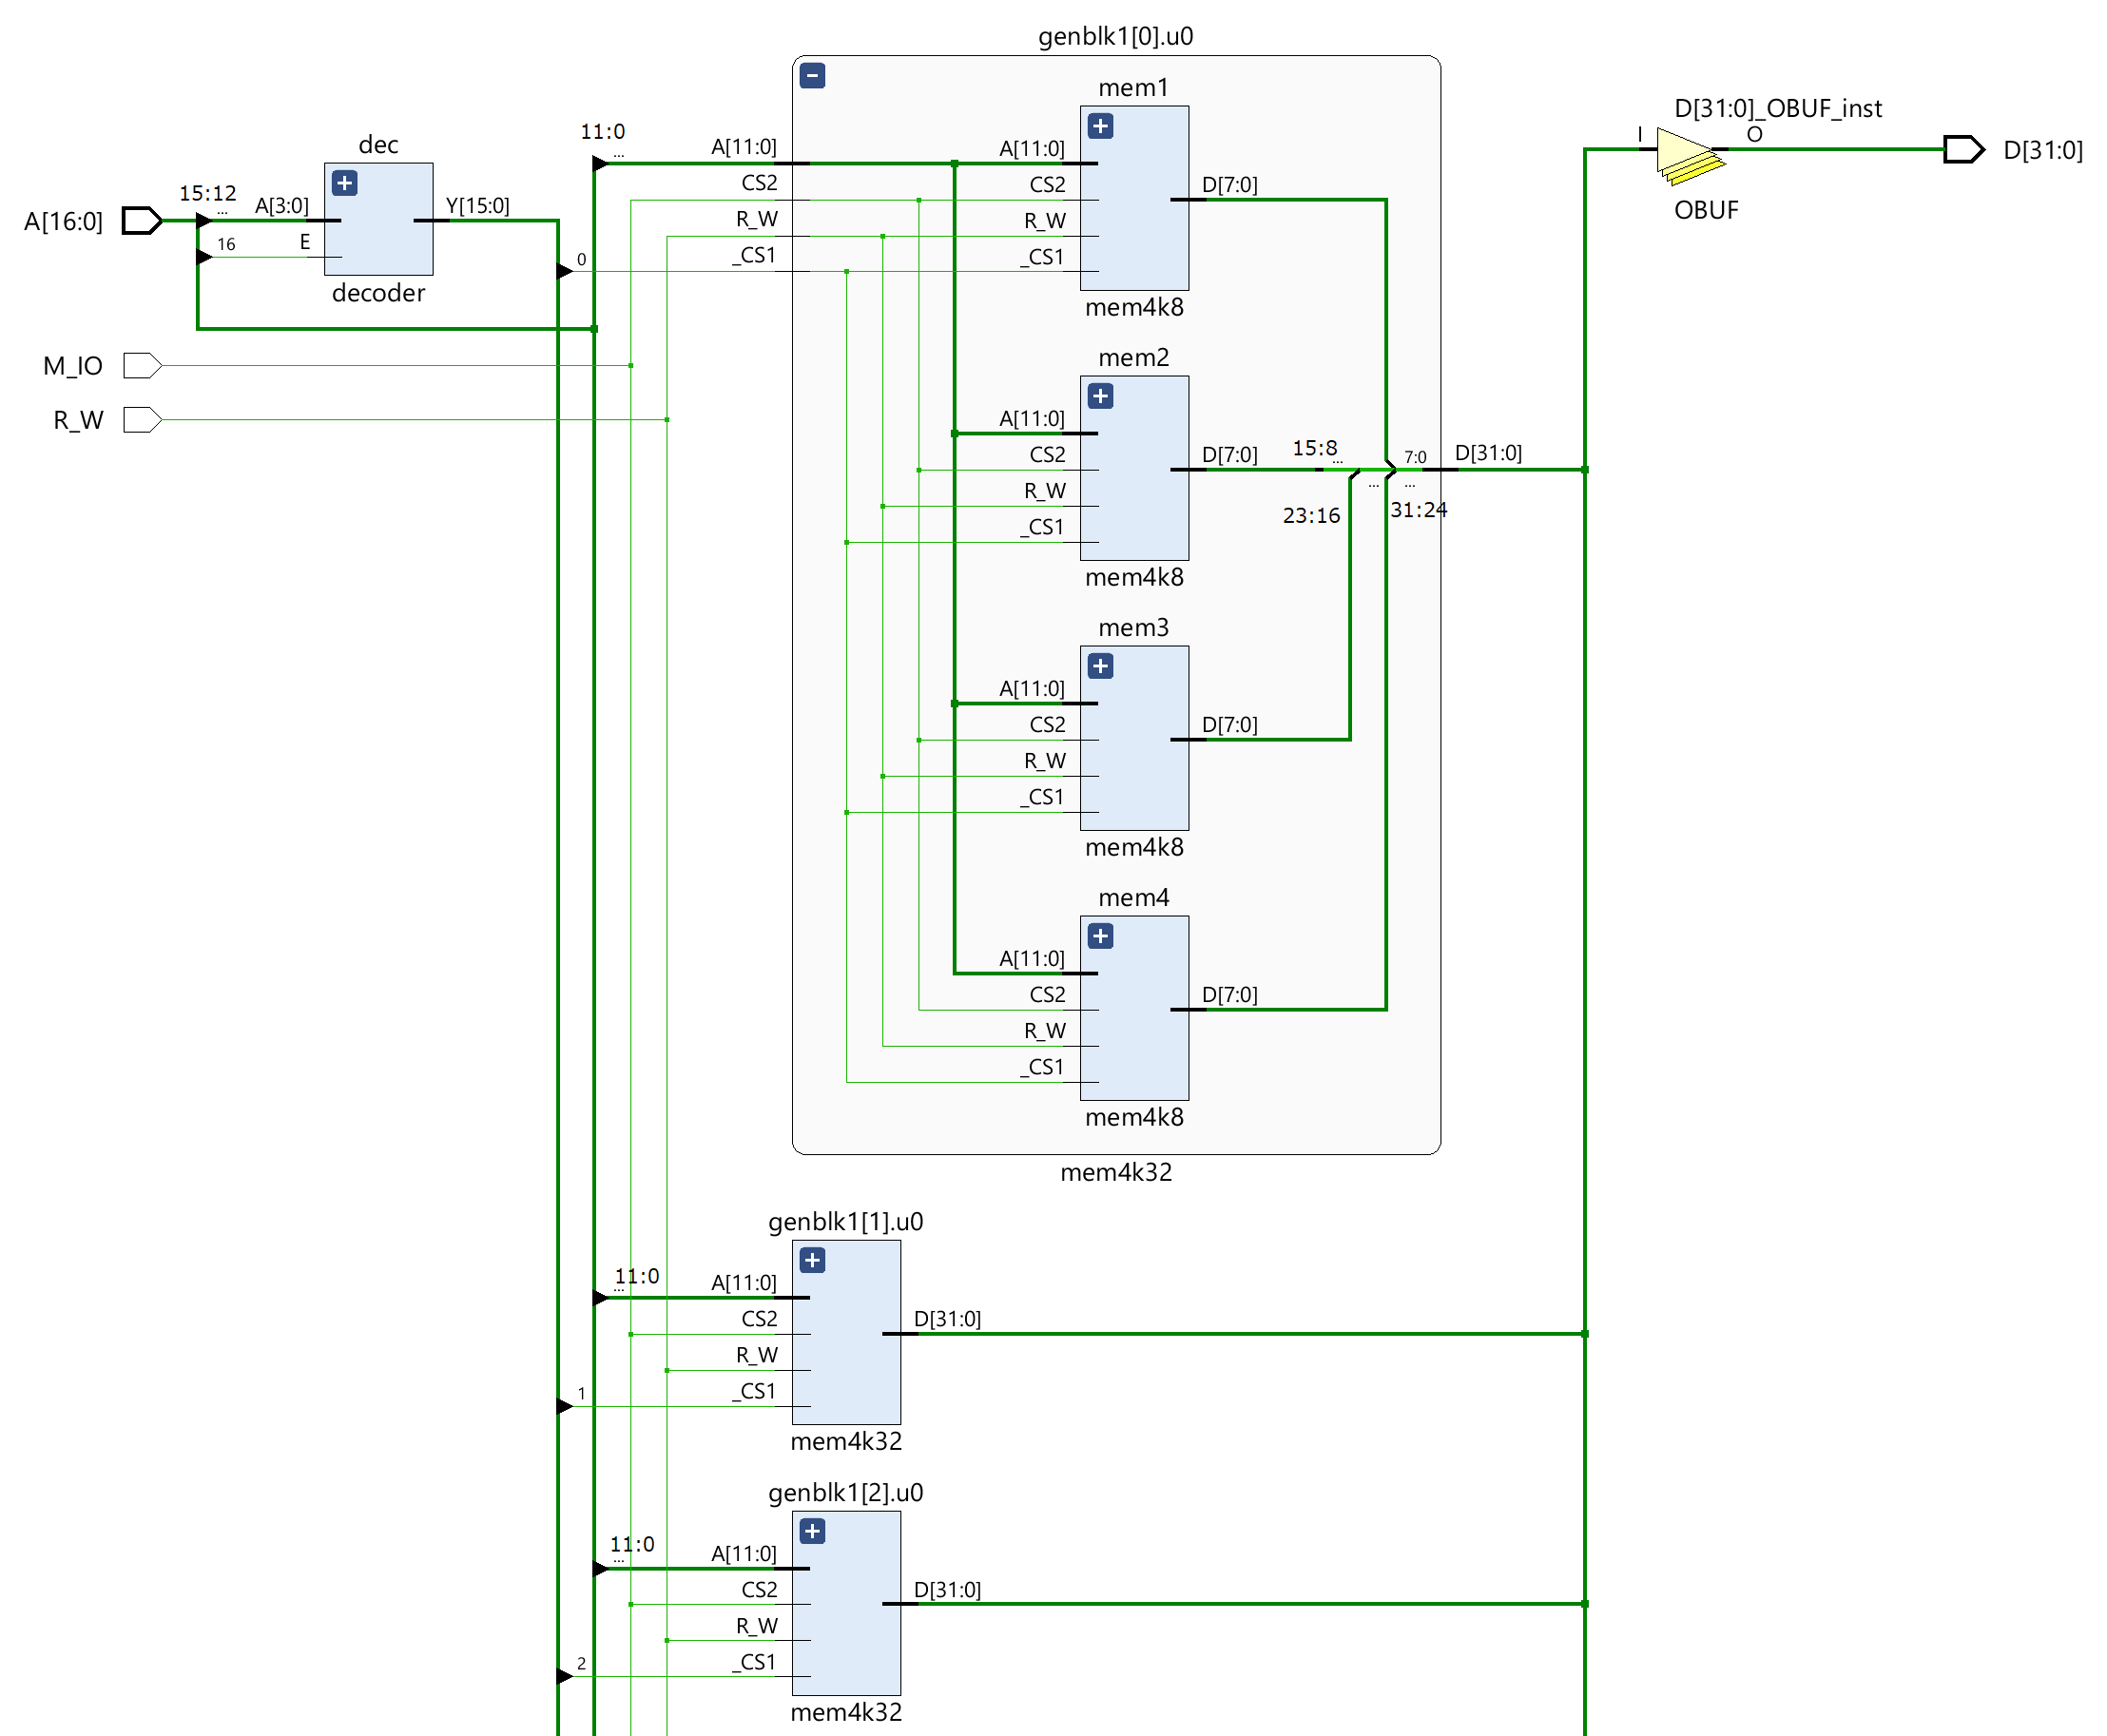
\includegraphics[width=\textwidth]{ECE3301_Assignment3_Zoomin.png}
  \caption{A portion of the below schematic denoting the distribution of split bus line omitted in original schematic generated by Xilinx Vivado}
\end{figure}


\newpage
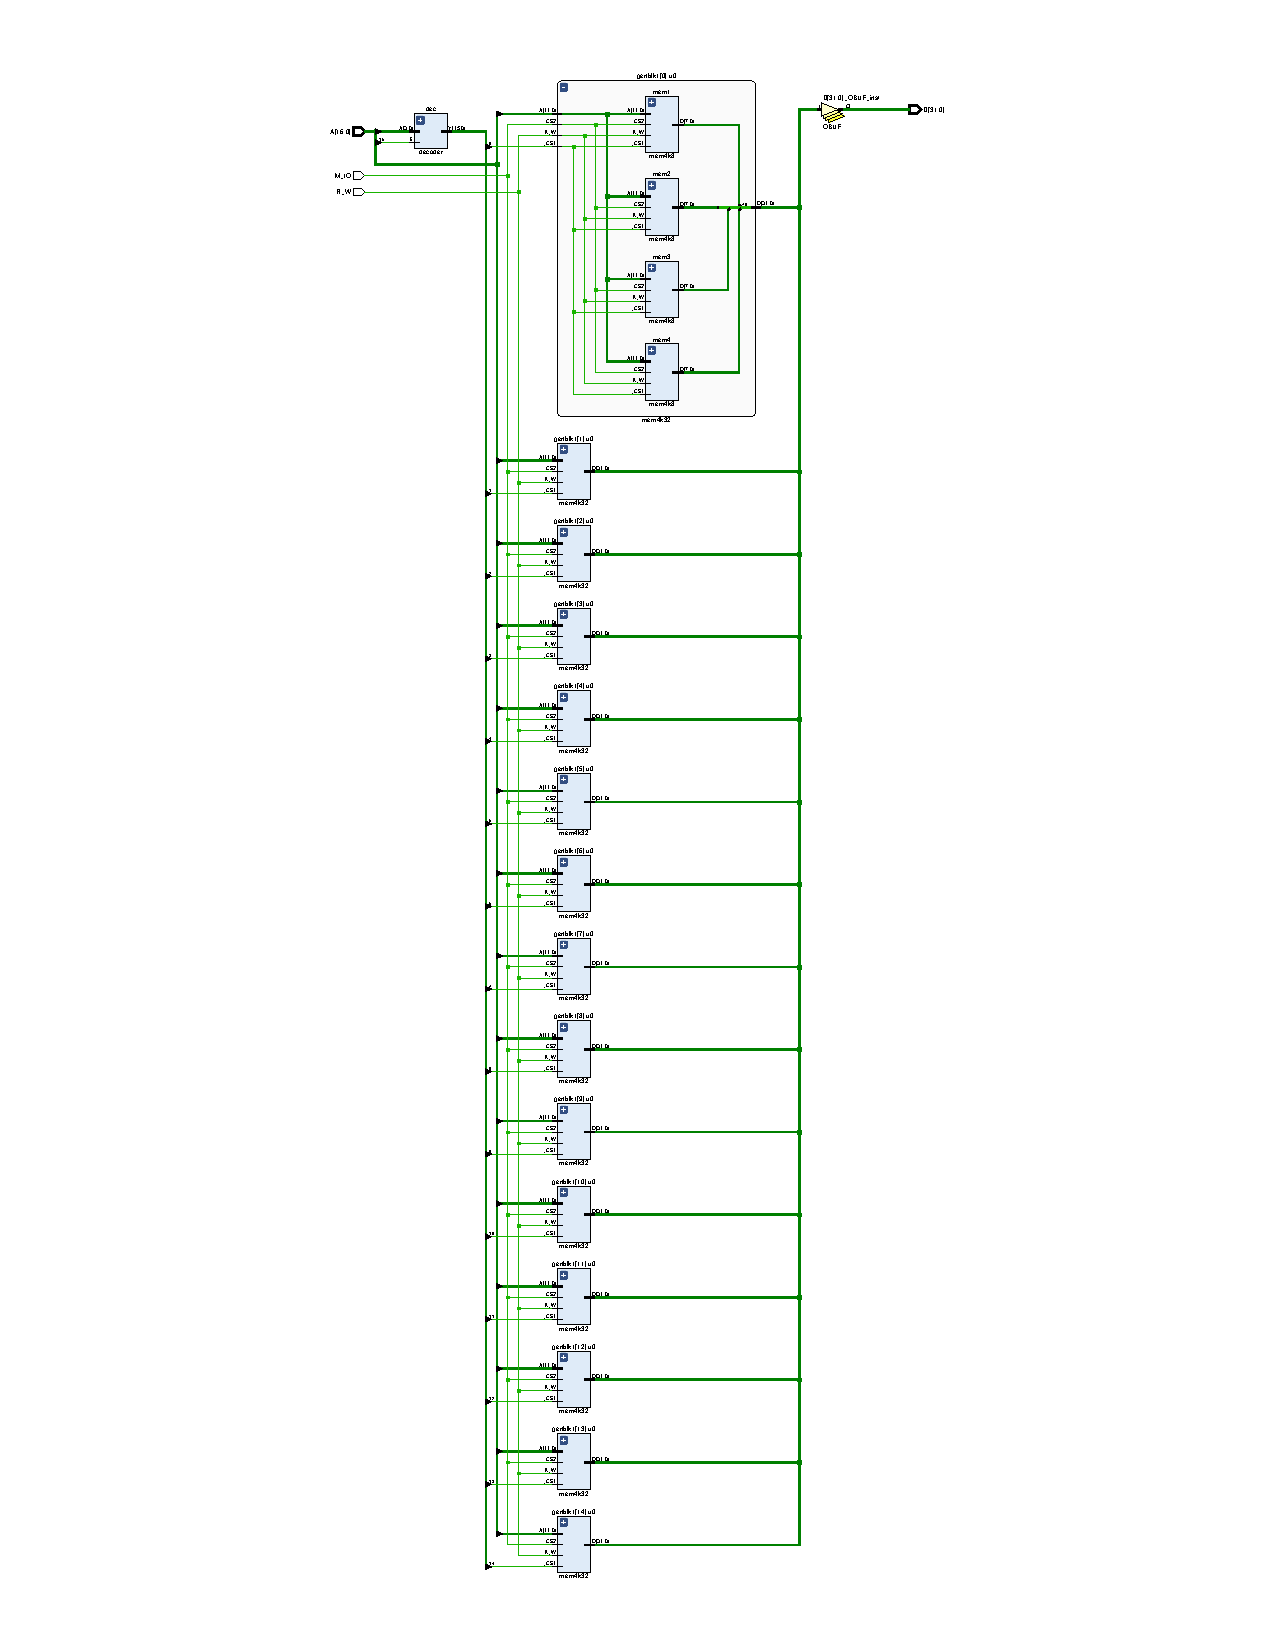
\includepdf[]{schematic.pdf}

\end{document}
